\section{Introduction}

Key value grouping operation, known as GROUP BY clause, is a key operation in database systems \cite{gray1997data}, \cite{stephens2005oracle}, \cite{mysql2009mysql}, \cite{momjian2001postgresql}. It groups a set of out-of-order records into multiple groups according to a certain key. GroupBy operation is often used with aggregate functions which produces a single row of summary information for each group, e.g., GroupBy-Aggregate in SQL. GroupBy is also widely used in distributed computing frameworks for distributing and locating the data. MapReduce \cite{dean2008mapreduce} expresses the computational process as three phases: Map, Shuffle and Reduce. During the shuffle phase, the key-value pairs that have the same key are aggregated together to form a Map output file, and they are sent to the same Reduce processor where the final cluster-wide aggregation (reduction) is applied on them. The efficiency of the key-value grouping step is crucial to both relational databases and distributed computing systems.


%Another popular use case for key grouping is to accumulate state across the stream in distributed stream processing engines (DSPEs) such as Storm \cite{storm2013storm}, S4 \cite{neumeyer2010s4}, Smaza \cite{noghabi2017samza}. This grouping in DSPEs is usually implemented by partitioning the stream on a key \cite{nasir2015power}. The strategies that are used to route tuples in a stream toward available operators can be divided into two categories: key grouping for stateful operators where a stream of tuples is partitioned in several disjoint sub-streams depending on the values contained \cite{rivetti2015efficient} and shuffle grouping for stateless operators where each tuple of a stream can be randomly assigned to any available operator \cite{Rivetti2016Online}. However, all the above works are focused on how to route kv-pairs to available operators for alleviating load imbalance but ignoring local key value aggregation overhead at the receiver side. In fact, the execution time depends on not only stream partition but also local aggregation. Our work will focus on accelerating the local GroupBy aggregation in this paper.

There are two categories of GroupBy implementations in general, sort-based grouping and hash-based grouping. Basically, the \emph{sort-based grouping} makes the data records sorted in the order of the group key, so that the records with the same group key are located together. While the \emph{hash-based grouping} typically hashes key-value pairs to a hash table structure where multiple key-value pairs in the same group (sharing the same group key) are stored in the same bucket.

Recall that key-value pairs (kv-pairs) grouping operation is the key operation in Hadoop MapReduce \cite{dean2008mapreduce}. The map output kv-pairs are locally grouped by keys before they are shuffled to reduce workers. These map output kv-pairs (i.e., reduce input kv-pairs) from various map workers are further merged to obtain a global grouped kv-pairs. Each group of kv-pairs sharing the same key is the input of a reduce function. In Hadoop Mapreduce implementation, a kind of sort-based grouping, \emph{merge-sort grouping}, is used, which can perform quite general grouping tasks at scale even in the absence of available memory. However, merge-sort grouping involves large amount of redundant computation and I/Os. The previous work \cite{shvachko2010hadoop,yu2009distributed,Li2011A} shows that merge-sort grouping adopted by Hadoop is found to be among the worst-performing choices.

For many applications, hash-based grouping is adopted because these applications require only unsorted grouping \cite{lin2011tenzing}, \cite{yu2009distributed}. However, hash-based grouping consumes more memory than sort-based grouping because it requires to load all records into memory. The performance heavily depends on the amount of available memory. A variant of hash grouping has been used in MariaDB \cite{bartholomew2012mariadb}, Oracle \cite{stephens2005oracle}, Postgresql \cite{momjian2001postgresql}, and SQL Server \cite{agrawal2005database}. It creates an in-memory hash table for grouping rows. If the hash table becomes too large to be fit in memory, the input records are partitioned into smaller work tables which are recursively partitioned until they fit into memory. Once all input groups have been processed, the completed in-memory groups are output and repeat the algorithm by reading back and aggregating one spilled partition at a time until all partitions have been processed. We refer to this approach as \emph{memory-constraint hash grouping}. It excels at efficiently aggregating large data sets and performs better than merge-sort grouping in some situations.

An alternate of hash grouping that can avoid memory overflow is using rehashing. The first hash grouping is applied to obtain coarse-grain kv-pair groups, where each group of kv-pairs covering multiple unique keys is written to a disk file. The second phase loads each kv-pairs file into memory and performs hash grouping on keys, so that the kv-pairs sharing the same key are grouped together in a bucket. These grouped kv-pairs are then written out for recycling memory to group next coarse-grain grouped kv-pairs (in next file). The number of files (coarse-grain groups) can be tuned according to available memory, and further optimizations can be applied to avoid memory overflow when processing each coarse-grain group. We refer to this approach as \emph{partitioned hash grouping}.

In addition, we can use an \emph{indexing-filling} approach that takes advantages from both sort grouping and hash grouping. A nice property of sort-based grouping is that the output file position of each group is determined before the grouping starts. While in hash-based grouping, the query of a specific group can be very fast. It first reads all data in one pass and evaluates the group size information associated for each key, which is maintained in an in-memory table. The output file offsets of all groups can be then calculated. In other words, the output kv-pairs are indexed in the first indexing phase. Then the data are parsed for the second time, and the kv-pairs are written out to specific file positions according to the offset table, which is the filling phase. Note that, the write operations can be cached to be sequential for I/O efficiency.

\begin{figure}[t]%figure 2
\subfloat[Performance comparison on big groups]{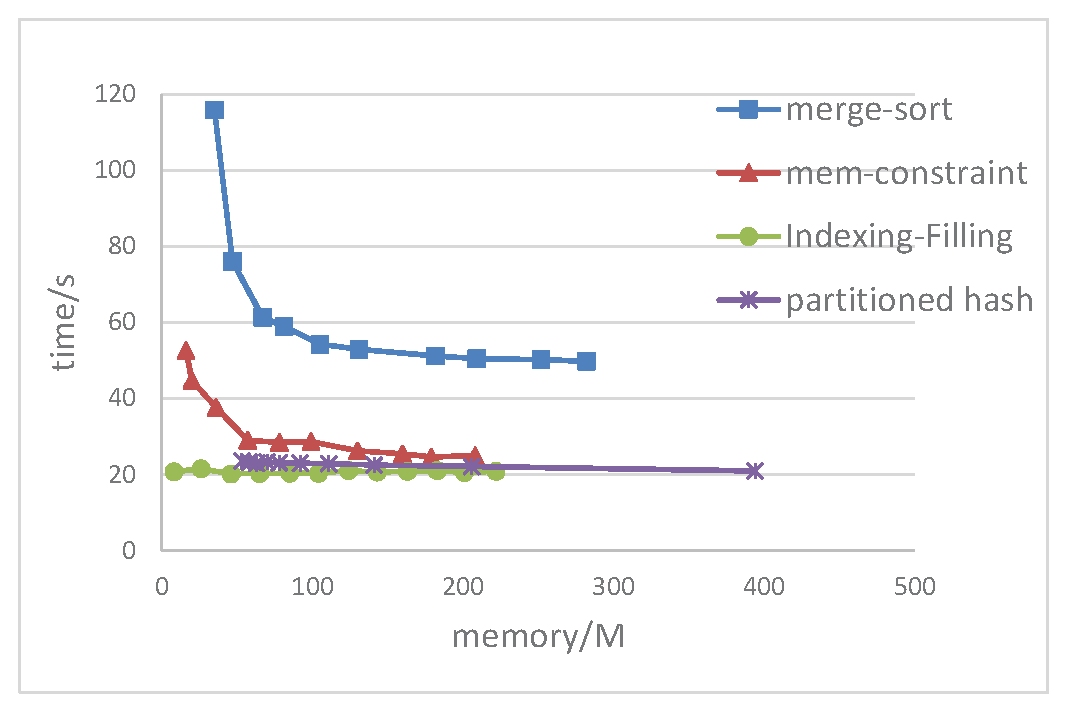
\includegraphics[width = 1.68in, height = 3.5cm]{fig/paretoBig.eps}\label{fig:paretoBig}}
    \hspace{0.23cm}
    \subfloat[Performance comparison on small groups]{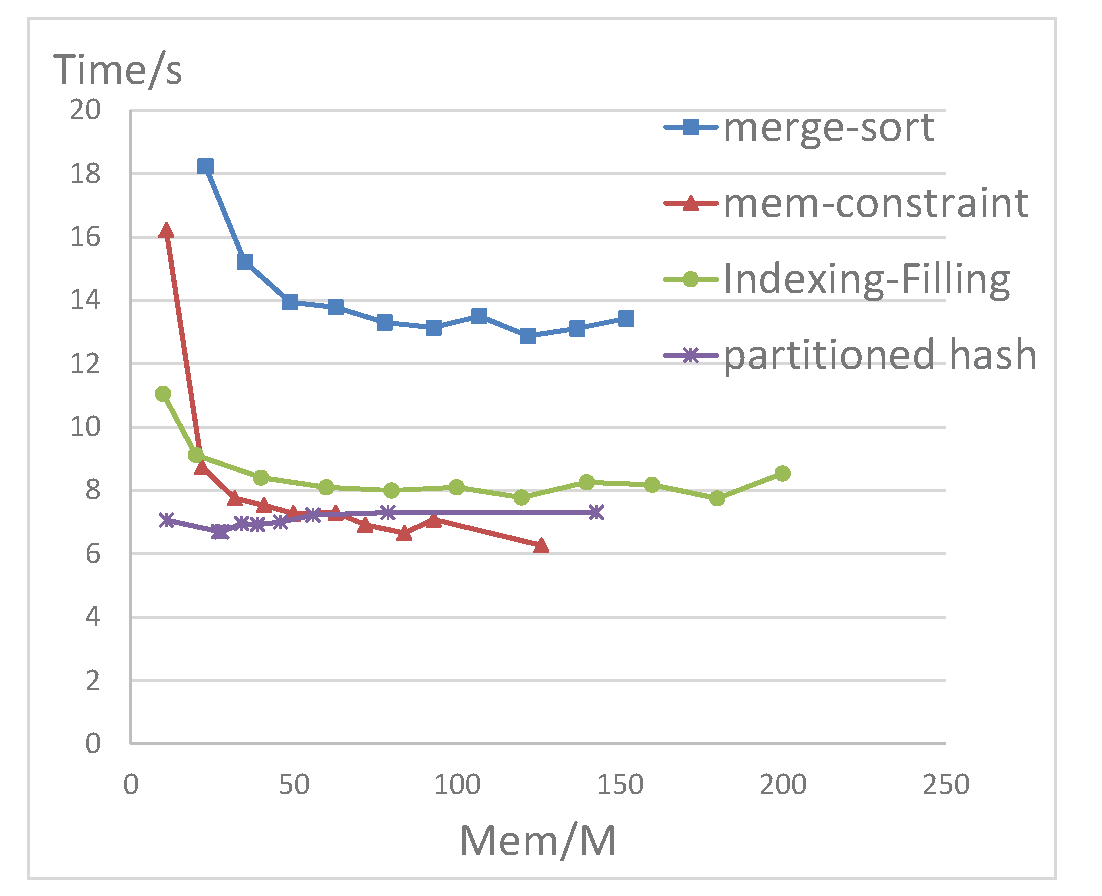
\includegraphics[width =1.68in, height = 3.5cm]{fig/paretoSmall.eps}\label{fig:paretoSmall}}\\
%\includegraphics[width=.5\textwidth]{fig/pareto_index_hash}
\caption{Performance comparison of big groups and small groups. The big groups and small groups are selected from a simulation data set Pareto, the group sizes of Pareto follow a power-law distribution.}
\label{fig: big and small}
\end{figure}

After reviewing these grouping algorithms, one question is raised. Which one is the best? Our observation is that no one wins all the time. As known, the group sizes in real data sets follow power-law distributions, the big group sizes and small group sizes vary over an enormous range. We further observe that these implementations exhibit different performance and memory efficiency for big groups and small groups. We extract the kv-pairs of big groups and small groups from a simulation data set Pareto (see Sec. \ref{} for dataset description) and evaluate the above four algorithms on grouping time and memory usage. It is obvious that using more memory will group data faster, so we show the results with both memory cost and runtime. With the same memory budget, the shorter runtime the better. The result for grouping big groups is shown in Figure \ref{fig:paretoBig}, where the indexing-filling method performs the best over the others. For big groups, it is likely to result in extremely large partitions that will be spilled to disk due to limited memory. This will incur multiple times of data exchanges between memory and disk, no matter for merge-sort grouping, memory-constraint hash, or partitioned hash. In this case, the indexing-filling approach is the most I/O effective one. On the other hand, for grouping small groups as shown in Figure \ref{fig:paretoSmall}, the hash based grouping approaches (memory-constraint hash and partitioned hash) perform better due to its fast location ability. In the case of processing extremely large input (i.e., with relatively small memory budget), the partitioned hash grouping runs faster with limited memory.




%When these data sets are processed by memory-constrain hash grouping in limited memory, the sub-tables sizes are not balanced caused by big groups, which leads to multiple recursive partitions and downgrade grouping performance. The performance reduction resulting from power-law distributions often occurs in various applications, we observe that these implementations exhibit different performance and memory usage for big groups and small groups. As shown in Figure \ref{fig:paretoBig}, the \emph{indexing and filling} method performs the best when grouping the big groups. Indexing and filling method proposed in this article is a file filling process according to an index, it creates an in-memory offset index which records each group's output position in result file firstly and fills the result file on the basis of the offset index, so the best grouping approach is indexing and filling for big groups. As shown in Figure \ref{fig:paretoSmall}, the \emph{partitioned hash grouping} method runs faster in limited memory when grouping small groups, that the kv-pairs in small groups are processed partition by partition is refered as partitioned hash grouping, so grouping small groups by partitioned hash is the best choice. Therefore, the ideal implementation should take the group size into account, and a hybrid grouping approach is desired.




Based on this observation, we propose an I/O efficient hash grouping scheme \emph{PowerHash} that leverages power-law property of the data group sizes. The big groups and small groups are processed separately. The kv-pairs of big groups are grouped by indexing-filling method, and the kv-pairs of small groups are grouped by the partitioned hash grouping approach. However, there is a key problem raised. How to estimate the group sizes efficiently and how to distinguish between the big groups and small groups? We use the count-min sketch \cite{Cormode2009Count} to approximately estimate the group sizes and identify the big groups and small groups. Given a memory budget, we comprehensively use indexing-filling grouping and partitioned hash grouping to group the data with the three-phase algorithm PowerHash. Our experimental results show that PowerHash always outperforms the other counterparts on real datasets. With the same memory cost, PowerHash is \textcolor{red}{25\%-100\%} times faster than the merge-sort grouping and \textcolor{red}{100\%-200\%} times faster than the memory-constraint hash grouping.

%The whole process of key grouping by power-law hash can avoid unnecessary repeat access to disk and needs less memory. When dealing with the big groups, the kv-pairs in big groups are written to the result file directly on the basis of offset index, only the offset index is stored in memory during the grouping process of big groups, the offset index size is much less than the big groups sizes and there is no need to load any whole group into memory, so the writing back to disk caused by out-of-memory can be prevented and the I/O cost can be reduced. For a data set whose group sizes follow a power-law distribution, the majority of the data set has been written to the result file after dealing with the big groups. So partition unbalance can be avoided to a great extent because there is no big groups in the remaining data set when we partition the small groups, and then it can prevent multiple recursive division to the big partitions.

%Our main contributions can be summarized as follows:
\begin{comment}
\begin{list}{\labelitemi}{\setlength{\leftmargin}{5mm}\setlength{\itemindent}{0mm}
\setlength{\topsep}{0.5mm}\setlength{\itemsep}{2mm}\setlength{\parsep}{0mm}}
\item Firstly, we study the problem of key grouping in modern distributed processing engines and traditional relation databases.
\item Secondly, we present an I/O efficient hash grouping scheme that leverages the power-law distributions and hashing, which can complete the key grouping operation with less memory usage and time cost.
\item Thirdly, we evaluate our algorithm through extensive experiments. The results show that power-law hash improves the performance with the same limited memory usage compared to memory-constraint hash, the runntime gap is greater compared to merge-sort.
\end{list}
\end{comment}

The rest of this paper is organized as follows. Section \uppercase\expandafter{\romannumeral2} describes the related work. In Section \uppercase\expandafter{\romannumeral3}, we propose our grouping method power-law hash and present the key optimizations. Section \uppercase\expandafter{\romannumeral4} discusses the parameters setting. The experimental results are presented in Section \uppercase\expandafter{\romannumeral5}. Finally, Section \uppercase\expandafter{\romannumeral6} concludes the paper.

